%%%%%%%%%%%%%%%%%%%%%%%%%%%%%%%%%%%%%%%%%%%%%%%%%%%%%%%%%%%%%%%%%%%
% Background
% Team:
% Wolverine
% Members: 
% Eric Lee, Jacky Wu, Karthick Mani, 
% Eric Chang, Dexter Chen, Peter Chen
% Relative files:
% Background_Wolverine.tex, Library.bib, WolverineChart.png
% Note: 
% Do not compile this file compile Main.tex to get the pdf file instead.
%%%%%%%%%%%%%%%%%%%%%%%%%%%%%%%%%%%%%%%%%%%%%%%%%%%%%%%%%%%%%%%%%%%
	
\subsection{Information retrieval on existing database}
\textit{\footnotesize Author:Dexter Chen, Eric Chang, Eric Lee, Jacky Wu, Karthick Mani, Kenvin Lo, Yu-cheng Chen.}\\

We live in the time where technologies evolve beyond our imagination. Due to the rapidly increasing amount of information, we can't rely on the old fashion ways to find data. We need new information retrieval methods to handle such a big amount of data. But most of the information retrieval methods such as search engine can't really search everything on the web. They can only search the data that has been captured into the database according to \cite{Grehan}. Thus, we need to create a database to store these data and automatically update them frequently.

There are several databases 



%\begin{figure*}[h!]
\begin{wrapfigure}{i}{\textwidth}
	\begin{center}
		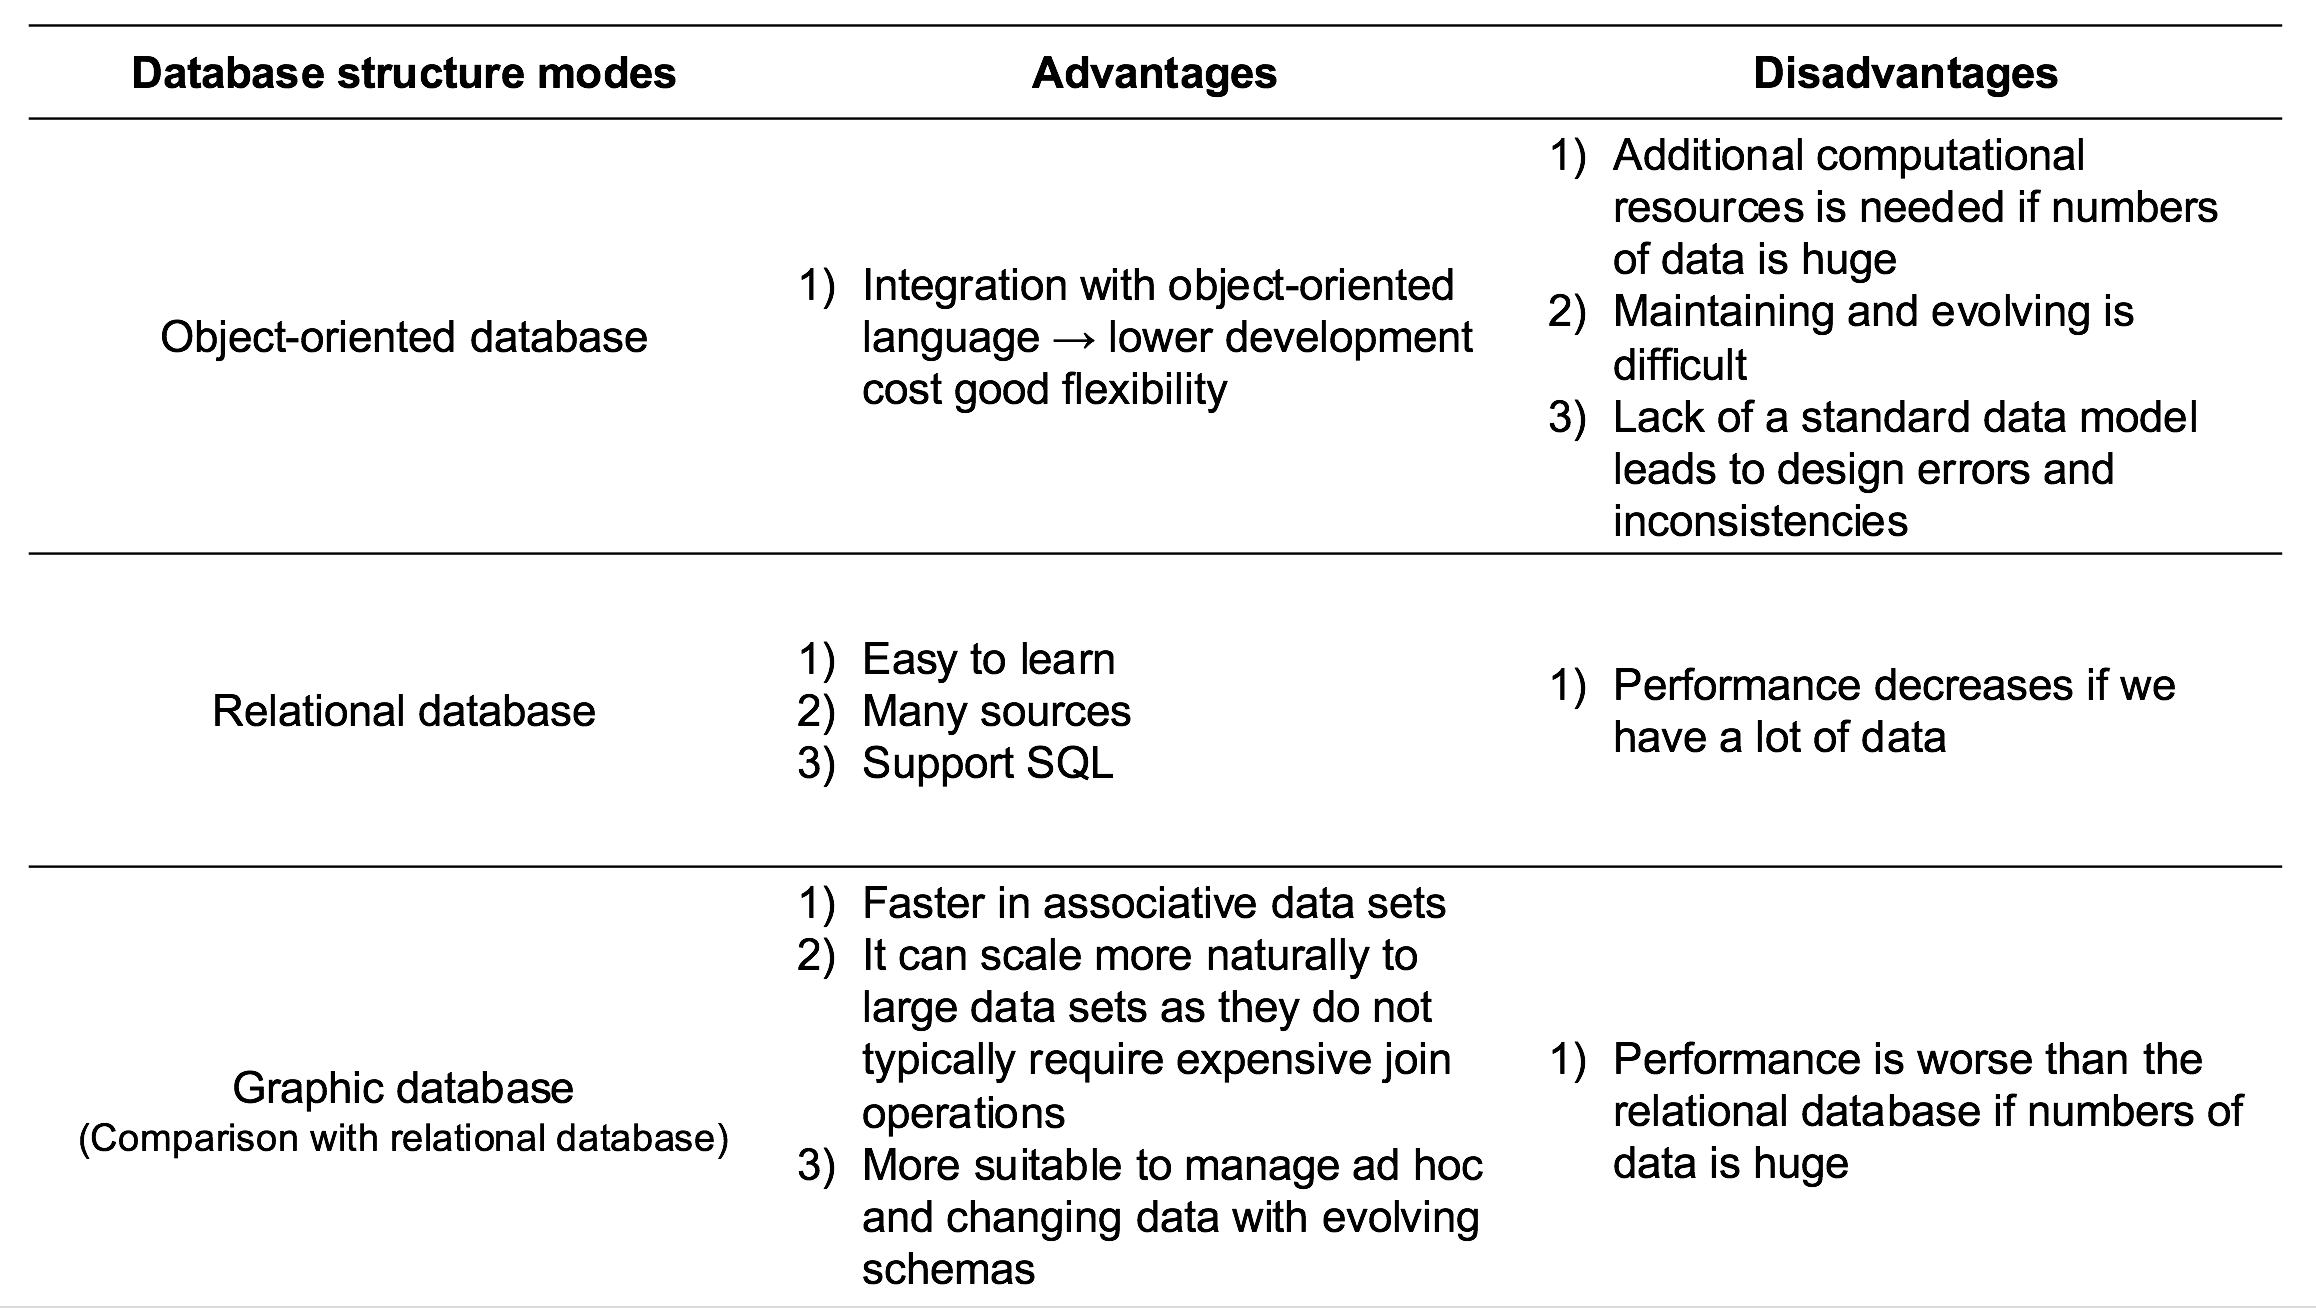
\includegraphics[width=0.8\textwidth]{WolverineChart2}
	\end{center}
	\caption{Database structure modes}
\end{wrapfigure}
%\end{figure*}
\clearpage
